\chapter{Introdução}
\label{cha:introducao}

A idéia de preservação de contorno e variação de intervalos entre
notas é encontrada em diferentes situações musicais. Há adequação de
notas à tonalidade em respostas tonais de fugas, em mudanças de modo
em peças do tipo tema e variações, e em \eng{leitmotifs} e idéias
fixas, citando apenas exemplos óbvios
\cite[p. 29]{morris87:composition}. Outras obras têm motivos cujos
intervalos são pouco a pouco expandidos ou contraídos, como por
exemplo ocorre no início da \opus{Música para Cordas, Percussão e
  Celesta}, de Béla Bartók.

Teóricos musicais reconhecem que ouvintes têm maior acuidade na
percepção de semelhança de contornos do que na semelhança de
alturas. Por isso novas teorias para comparação de contornos se
tornaram necessárias à área da Análise Musical
\cite[p. 226]{marvin.ea87:relating}.

Há diversas definições de contorno melódico na literatura
\cite{piston59:harmony,toch77:shaping,schonberg:fundamentals,adams76:melodic,marvin.ea87:relating,morris87:composition,clifford95:contour,beard03:contour},
cada uma delas relacionada com o objetivo do trabalhos de seu
autor. No presente estudo entendemos que contorno melódico é um
conjunto ordenado de alturas de notas (chamadas de pontos) cujo valor
absoluto é ignorado e somente o registro, que pode ser mantido ou
variar ascendente e descendentemente entre um ponto e outro, é
considerado.

O estudo de contornos é importante porque, assim como conjuntos de
notas e motivos, contornos ajudam a dar coerência musical a uma
obra. Eles representam estruturas musicais manipuláveis através de
várias operações como inversão e retrogradação, e podem ser abordados
tanto do ponto de vista da análise quanto da composição.

No campo da percepção musical contorno melódico é uma importante
característica para o reconhecimento de melodias familiares \cite[p.
136]{dowling.ea86:music}. Além disso é reconhecido que ouvintes têm
maior acuidade na percepção de semelhança de contornos do que na
semelhança de alturas. Por isso novas teorias para comparação de
contornos se tornaram necessárias à área da Análise Musical
\cite[p. 226]{marvin.ea87:relating}.

\chapter{Sobre contornos}
\label{cha:sobre-contornos}

%% brainstorm

% análise: comparação e equivalência de materiais.
% análise: objetivos diferentes.
% redução: tipologia de adams e algoritmo de morris
% equivalência a partir de matriz de comparação
% cognição: dowling
% terminologias diferentes: friedmann
% problemas com teorias: clifford
% estruturação da composição a partir de contornos
% exemplos com análise de peças?
% contornos: coerência, schoenberg

%% lembrete: falar que não abordaremos o aspecto duração

%% lembrete: falar que consideramos operação tudo o que parte do
%% contorno: subconjuntos, retrógrado, int, etc

Teorias que visam sistematizar o estudo de contornos dispõem de várias
operações para mapeamento e comparação de contornos
\cite{friedmann85:methodology,friedmann87:response,morris87:composition,morris93:directions,marvin.ea87:relating,clifford95:contour,polansky.ea92:possible,quinn97:fuzzy,beard03:contour}
\note{período fragmentado}. A partir das idéias destas teorias é
possível, por exemplo, reconhecer semelhanças entre as duas melodias
de quatro notas da figura \ref{fig:ly-cseg-5968}, cujo contorno está
representado em gráfico cartesiano na figura
\ref{fig:cseg-5968}. Outros exemplos de melodias de contornos
semelhantes podem ser vistos nas figuras \ref{fig:melodias-cseg} e
\ref{fig:graficos-cseg}.

\begin{figure}
  \centering
  \subfloat[melodias com cseg $P\langle5\:9\:6\:8\rangle$]{
    \includegraphics[scale=.9]{ly-5968}
    \label{fig:ly-cseg-5968}
  }
  \subfloat[melodias com cseg $Q\langle5\:7\:6\:8\rangle$]{
    \includegraphics[scale=.9]{ly-5768}
    \label{fig:ly-cseg-5768}
  }

  \subfloat[melodias com cseg $R\langle3\:0\:5\:1\rangle$]{
    \includegraphics[scale=.9]{ly-3051}
    \label{fig:ly-cseg-3051}
  }
  \caption{Melodias para diferentes cseg}
  \label{fig:melodias-cseg}
\end{figure}

\begin{figure}
  \centering
  \subfloat[cseg $P\langle5\:9\:6\:8\rangle$]{
    \includegraphics{c-5968}
    \label{fig:cseg-5968}
  }
  \subfloat[cseg $Q\langle5\:7\:6\:8\rangle$]{
    \includegraphics{c-5768}
    \label{fig:cseg-5768}
  }
  \subfloat[cseg $R\langle3\:0\:5\:1\rangle$]{
    \includegraphics{c-3051}

    \label{fig:cseg-3051}
  }
  \caption{Gráficos de cseg}
  \label{fig:graficos-cseg}
\end{figure}

A música pode ser entendida a partir de \note{``entendida a partir de
  espaços'' fica estranho, que tal ``visualizada em''?} diferentes
espaços, como de altura e de contorno \cite{morris87:composition}. O
espaço de contorno (\tr{c-space}) é uma abstração de espaço musical
que consiste em elementos organizados do grave para o agudo
desconsiderando os intervalos exatos entre eles. Leva-se em conta
apenas a relação entre os registros dos elementos. O \tr{c-space} pode
ser entendido como um grande conjunto de \tr{c-pitch} (alturas de
contorno).

Cada conjunto de \tr{c-pitch} contido em um \tr{c-space} é chamado de
\tr{cseg} (segmento de contorno)\footnote{Trata-se de uma idéia
  semelhante à da geometria, de reta e segmento de reta, onde o
  \tr{c-space} seria análogo à reta, e o \tr{cseg} ao segmento de
  reta.}. Estes \tr{cseg} podem conter elementos contíguos ou não do
\tr{c-space}. Subconjuntos de \tr{cseg} são chamados \tr{csubseg}. A
figura \ref{fig:c-space} contém três exemplos de um mesmo \tr{c-space}
de 10 \tr{c-pitch} enumerados do mais grave (0) para o mais agudo
(9). Na figura \ref{fig:c-space5968} o \tr{c-space} contém o \tr{cseg}
P, com os \tr{c-pitch} 5, 9, 6 e 8. Na figura \ref{fig:c-space7420} o
\tr{c-space} contém o \tr{cseg} M, com \tr{c-pitch} 7, 4, 2 e 0. Ainda
nesta figura o \tr{cseg} M contém o \tr{csubseg} O, com \tr{c-pitch} 4
e 2. Por último, na figura \ref{fig:c-space564} o \tr{c-space} contém
o \tr{cseg} N, com os \tr{c-pitch} não adjacentes 5, 6 e 4.

\begin{figure}
  \centering
  \subfloat[Cseg P]{
    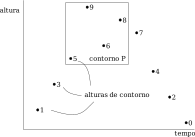
\includegraphics[scale=.97]{cspace-5968}
    \label{fig:c-space5968}
  }
  \subfloat[Cseg M e csubseg O]{
    \includegraphics[scale=.97]{cspace-7420}
    \label{fig:c-space7420}
  }
  \subfloat[Cseg N]{
    \includegraphics[scale=.97]{cspace-564}
    \label{fig:c-space564}
  }
  \caption{C-space com cseg e csubseg}
  \label{fig:c-space}
\end{figure}

Por definição contornos são ordenados no tempo, representados por
letras maiúsculas e têm seus elementos representados por numerais
subscritos. Estes numerais indicam a posição destes elementos em ordem
temporal \cite{marvin.ea87:relating}. Por exemplo, um contorno $P$ de
quatro elementos tem a seguinte configuração: $P\:\langle
P_0\:P_1\:P_2\:P_3\rangle$. Dessa forma, dado um contorno
$P\:\langle5\:9\:6\:8\rangle$, $P_0$ é igual a 5, $P_1$ é igual a 9,
$P_2$ é igual a 6, e $P_3$ é igual a 8.

Operações como retrogradação e rotação são semelhantes às realizadas
com alturas de notas. A expansão de intervalos \note{acho legal deixar
  mais claro o que é a expansão de intervalos, talvez com um exemplo}
consiste na multiplicação de cada \tr{c-pitch} por um dado fator.

A operação de inversão de um contorno $P$ de ordem $q$ é representada
por $IP$, e é matematicamente calculada por
$IP_n=(q-1-P_n)$. Portanto, dado um \tr{cseg}
$P\:\langle5\:9\:6\:8\rangle$ (de ordem 10), $IP_0=(10-1-P_0)$. Logo,
$IP_0=4$. Aplicando-se a mesma idéia aos outros elementos chegamos ao
contorno $IP\:\langle4\:0\:3\:1\rangle$. É possível ainda relacionar a
inversão entre elementos através da matriz de comparação. Calcula-se
esta inversão com a operação $COM(P_a,P_b)=-COM(IP_a,IP_b)$.

Relações de similaridade \cite{marvin.ea87:relating} são analisadas
com operações como comparação (\tr{COM}), matriz de comparação
(\tr{COM-matrix}) e classe de contorno (\tr{CC}) \note{fica parecendo
  que matrizes de comparação e classes de contorno são operações, acho
  bom mudar a vírgula de lugar ou algo assim}.

A operação de comparação \tr{COM(a,b)} retorna a diferença de registro
entre dois elementos, ou seja, informa se um elemento é mais agudo,
mais grave ou de mesma altura que outro. O valor de \tr{COM} é o sinal
``$+$'' se $b$ é maior que $a$; ``$-$'' se $b$ é maior que $a$; e
``$0$'' se $b$ é igual a $a$. Por exemplo, no contorno
$P\:\langle5\:9\:6\:8\rangle$, o valor de $COM(P_0,P_1)$ é o sinal
``$+$'', o de $COM(P_1,P_2)$ é ``$-$'', e o valor de $COM(P_3,P_0)$ é
o sinal ``$+$''. Esta medida de comparação pode ser invertida de modo
que a comparação entre dois elementos é igual ao inverso da comparação
destes elementos em ordem reversa. Esta idéia pode ser melhor
entendida observando-se a equação $COM(a,b)=-COM(b,a)$.

A \tr{COM-matrix} é uma matriz bidimensional que compara um \tr{cseg}
com ele próprio. Esta matriz mostra os resultados da função de
comparação \tr{COM} para todos os \tr{c-pitch} de um \tr{cseg}. A
tabela \ref{tab:matriz-5968} contém a matriz de comparação de um
\tr{cseg} $P\:\langle5\:9\:6\:8\rangle$. As \tr{COM-matrix} dos
exemplos já vistos na figura \ref{fig:graficos-cseg} podem ser vistos
na tabela \ref{tab:matriz-exemplos}.

\begin{table}
  \centering
  \subfloat[cseg $P\langle5\:9\:6\:8\rangle$]{
    \begin{tabular}{c|cccc}
      & $5$ & $9$ & $6$ & $8$ \\
      \hline
      $5$ & $0$ & $+$ & $+$ & $+$ \\
      $9$ & $-$ & $0$ & $-$ & $-$ \\
      $6$ & $-$ & $+$ & $0$ & $+$ \\
      $8$ & $-$ & $+$ & $-$ & $0$
    \end{tabular}
    \label{tab:matriz-5968}
  }
  \qquad
  \subfloat[cseg $Q\langle5\:7\:6\:8\rangle$]{
    \begin{tabular}{c|cccc}
      & $5$ & $7$ & $6$ & $8$ \\
      \hline
      $5$ & $0$ & $+$ & $+$ & $+$ \\
      $7$ & $-$ & $0$ & $-$ & $+$ \\
      $6$ & $-$ & $+$ & $0$ & $+$ \\
      $8$ & $-$ & $-$ & $-$ & $0$
    \end{tabular}
    \label{tab:matriz-5768}
  }
  \qquad
  \subfloat[cseg $R\langle3\:0\:5\:1\rangle$]{
    \begin{tabular}{c|cccc}
      & $3$ & $0$ & $5$ & $1$ \\
      \hline
      $3$ & $0$ & $-$ & $+$ & $-$ \\
      $0$ & $+$ & $0$ & $+$ & $+$ \\
      $5$ & $-$ & $-$ & $0$ & $-$ \\
      $1$ & $+$ & $-$ & $+$ & $0$
    \end{tabular}
    \label{tab:matriz-3051}
  }
  \caption{Exemplos de \tr{COM-matrix}}
  \label{tab:matriz-exemplos}
\end{table}

As diagonais superiores à diagonal principal zero da \tr{COM-matrix}
são chamadas de $INT_n$, onde $n$ é o número da diagonal: 1 para a
superior mais próxima da diagonal zero, 2 para a seguinte, 3 para a
posterior e assim por diante. A diagonal $INT_1$ traz comparações de
registros entre elementos adjacentes do \tr{cseg}. Em
$P\:\langle5\:9\:6\:8\rangle$, por exemplo,
$INT_1=\langle+\:-\:+\rangle$, ou seja, o movimento melódico é
ascendente entre 5 e 9, descendente entre 9 e 6, e ascendente entre 6
e 8. Esta comparação é feita também com uma operação conhecida como
série de contornos adjacentes (\tr{CAS}) \footnote{Em teorias de
  contornos não há consenso em relação a terminologia. Por isso há
  idéias semelhantes com nomes diferentes, como $INT_1$ e \tr{CAS}
  \cite{friedmann87:response}.}.

A classe de contorno (\tr{CC}) é uma operação importante para a
verificação de similaridade entre contornos. Obtém-se \tr{CC}
numerando-se ordenadamente todos os \tr{c-pitch} de $0$ a $(n-1)$,
sendo $n$ o número total de \tr{c-pitch} do \tr{cseg}. Uma \tr{CC}
engloba todos os contornos considerados equivalentes. Dois ou mais
contornos são considerados equivalentes quando geram uma mesma
\tr{COM-matrix}, ou seja, quando mantêm a mesma estrutura de registro
entre suas notas. Dessa forma, dado um \tr{cseg}
$P\:\langle5\:9\:6\:8\rangle$, são considerados seus equivalentes os
\tr{cseg} $\langle1\:5\:2\:3\rangle$, $\langle0\:10\:4\:7\rangle$,
$\langle0\:3\:1\:2\rangle$ e muitos outros. Todos eles têm
$\langle0\:3\:1\:2\rangle$ como forma normal e \tr{CC}.

Os Intervalos de Contorno (\tr{CI}) representam as relações entre
\tr{c-pitch} de uma \tr{CC} e podem ser entendidos de duas formas:
guardando o valor entre os \tr{c-pitch}
\cite{friedmann85:methodology}, ou guardando apenas a direção, mas não
o valor da diferença entre os \tr{c-pitch}
\cite{morris93:directions}. Por exemplo, para um mesmo \tr{cseg}
$P\:\langle0\:3\:1\:2\rangle$, o \tr{CI} entre $P_1$ e $P_2$ para
Friedmann é -2, e para Morris, ``$-$''.

O Vetor de Intervalos de Contornos (\tr{CIA}) descreve a freqüência de
cada tipo de \tr{CI} em uma \tr{CC}. Por exemplo, o \tr{cseg}
$P\:\langle0\:3\:1\:2\rangle$ tem \tr{CIA}
$\langle2,1,1/1,1,0\rangle$. Os dígitos da esquerda da barra
representam os \tr{CI} ascendentes em ordem crescente, e os dígitos da
direita os \tr{CI} descendentes em ordem crescente de valor
absoluto. \cite{friedmann85:methodology}. Os Vetores de classe de
contorno (\tr{CCVI} e \tr{CCVII}), de dois dígitos cada um, refletem
os movimentos ascendentes e ascendentes de um contorno e são
calculados a partir dos \tr{CI} ascendentes e descendentes.

A redução de contornos é possível a partir de dois diferentes
algoritmos \cite{adams76:melodic,morris93:directions}. O algoritmo de
Adams, criado para definir uma tipologia de contornos, reduz uma
melodia inteira a apenas quatro \tr{c-pitch}\footnote{Adams utiliza
  uma terminologia diferenciada da que apresentamos aqui.}: a primeira
altura, a última, a mais aguda e a mais grave. O algoritmo de Morris,
processado em várias etapas, reduz a melodia através da observação de
mudanças de direção entre segmentos adjacentes e eliminação de
\tr{c-pitch}.

%% texto antigo

Teorias de contornos foram desenvolvidas primariamente como técnicas
analíticas para composições atonais que podem não ter características
musicais usadas para demonstrar coerência em composições tonais
\cite[p. 1]{beard03:contour}.

Embora teorias de contorno não tenham surgido para análise de obras
tonais, a análise a partir da perspectiva dos contornos já se mostrou
eficiente também neste tipo de obra. Assim, além de obras de Schönberg
\cite{friedmann85:methodology} e Webern \cite{clifford95:contour},
sonatas para piano de Mozart \cite{beard03:contour} já foram
analisadas sob a ótica das teorias de contornos.

Contorno é um conjunto ordenado de elementos distintos, com ou sem
repetição, numerados de forma ascendente
\cite[p. 206]{morris93:directions}. Por definição contornos musicais
são ordenados \cite[p. 228]{marvin.ea87:relating}.

Um contorno pode ser interpretado como registro, dinâmica ou densidade
de acordes no tempo \cite[p. 206]{morris93:directions}
\cite[p. 22]{clifford95:contour}. Podemos ver representações do
contorno \contorno{4\:3\:5\:6} na figura
\ref{fig:non-melodic-contours}.

\begin{figure}
  \centering
  \subfloat[alturas no tempo]{
    \includegraphics[scale=1]{pitches-in-time}
    \label{fig:pitches-in-time}}
  \subfloat[densidade de acordes no tempo]{
    \includegraphics[scale=1]{chord-densities-in-time}
    \label{fig:chord-densities-in-time}}

  \subfloat[dinâmicas no tempo]{
    \includegraphics[scale=1]{dynamics-in-time}
    \label{fig:dynamics-in-time}}
  \caption{Contornos \contorno{4\:3\:5\:6} não melódicos}
  \label{fig:non-melodic-contours}
\end{figure}

Adams propôs uma tipologia de contornos melódicos para classificação
de melodias indígenas americanas. Esta tipologia está baseada na
redução do contorno de cada melodia a quatro pontos --- nota inicial
(I), nota final (F), nota mais aguda (H) e nota mais grave (L) --- e
na classificação da inclinação entre essas notas. A inclinação entre
as notas pode ser ascendente, descendente ou nula, e repetição de
notas são admitidas. Adams propôs 15 tipos de contornos melódicos,
como se vê na figura \ref{fig:adams-typology}. A inclinação (ou
\eng{slope}) entre a nota inicial e final é indicada por $S1$ ($I >
F$), $S2$ ($I = F$) e $S3$ ($I < F$). A mudança de direção (ou
\eng{deviation}) é indicada por $Dø$ (sem mudança de direção), $D1$
(se H ou L são diferentes de I ou F) e $D2$ (se H e L são diferentes
de I e F). A ordem entre as mudanças de direção, chamada
\eng{reciprocal}, é indicada por $R1$ (H antes de L) e $R2$ (L antes
de H) \cite{adams76:melodic}.

\begin{figure}
  \centering
  \includegraphics[scale=.6]{adams-typology}
  \caption{Tipologia de contornos de Charles Adams}
  \label{fig:adams-typology}
\end{figure}

A terminologia utilizada em teorias de contornos melódicos não é
uniforme. Cada autor utiliza termos diferentes para operações
semelhantes \cite{friedmann87:response}. A tabela
\ref{tab:compara-ferramentas} tem uma comparação dos termos usados por
Friedmann, e Morris, Marvin e Laprade.

\begin{table}
  \centering
  \begin{tabular}{l|l}
    Friedmann & Marvin e Laprade \\ \hline
    \eg{cas}  & INT$_1$ \\
  \end{tabular}
  \caption{Quadro comparativo de ferramentas de análise de contornos}
  \label{tab:compara-ferramentas}
\end{table}

Morris define os conceitos de espaço de alturas (\eg{p-space}) e
espaço de contorno (\eg{c-space}) \cite{morris87:composition}. Em
\eg{p-space} os elementos a serem considerados são as notas e em
\eg{c-space} os elementos são os registros dessas notas. Beard
confunde a idéia de espaço do contorno com a definição de classe de
contorno \cite[p. 11]{beard03:contour}.

A Matriz de Comparação (\eg{com-matrix}) representa o total de
comparações de um contorno. É obtida através da comparação de todos os
pares ordenados de um contorno. Em uma matriz Mi de um contorno $P$, a
posição $E (x,y)$ contém $Com (Px,Py)$. A matriz exibe uma simetria de
sinais invertidos em torno da diagonal principal, esta preenchida
apenas por zeros. Um exemplo desta matriz referente ao contorno
$\langle 4\:3\:5\:6 \rangle$ pode ser visto na tabela
\ref{fig:matriz-4356} \cite[p. 28]{morris87:composition}.

\begin{figure}
  \centering
  \begin{tabular}{r|cccc}
    & $4$ & $3$ & $5$ & $6$ \\
    \hline
    $4$ & $0$ & $-$ & $+$ & $+$ \\
    $3$ & $+$ & $0$ & $+$ & $+$ \\
    $5$ & $-$ & $-$ & $0$ & $+$ \\
    $6$ & $-$ & $-$ & $-$ & $0$ \\
  \end{tabular}
  \caption{Matriz de comparação do contorno $\langle 4\:3\:5\:6 \rangle$}
  \label{fig:matriz-4356}
\end{figure}

Cada diagonal à direita da diagonal zero recebe o nome INT$_n$, onde
$n$ representa a diferença de posição entre dois elementos. Dessa
forma INT$_1$ representa as diferenças de altura entre \eg{cps}
adjacentes, INT$_2$ representa as diferenças de altura entre
\eng{c-pitches} separados não adjacentes separados por um elemento e
assim por diante \cite[p. 231]{marvin.ea87:relating}. Dado um contorno
$\langle 4\:3\:5\:6 \rangle$, INT$_1 = \langle - + +\rangle$
representa as diferenças entre $4$ e $3$, $3$ e $5$, e $5$ e
$6$. INT$_2 = \langle + + \rangle$ representa as diferenças entre $4$
e $5$, e $3$ e $6$.

Esta matriz permite a verificação de duas classes de equivalência de
contornos. A primeira é formada por todos os \eg{cseg} que dividem uma
mesma \eg{com-matrix}, e a segunda --- \eg{csegclass} --- formada por
todos os \eg{cseg} relacionados por operações de identidade,
translação, retrogradação, inversão e retrogradação da inversão.

A operação de inversão é obtida pela subtração de todos os \eg{cps}
por $(n-1)$. Para um dado \eg{cseg} $P$, a operação de identidade é
identificada como $IP$. A retrogradação de um \eg{cseg} $P$
(representado por $RP$), bem como de sua inversão ($IP$) são obtidas
colocando os \eg{cps} em ordem reversa
\cite[p. 231]{marvin.ea87:relating}.

A forma prima de um \eg{cseg} é obtida operando-se de um algoritmo de
três etapas:
\begin{enumerate}
\item realiza-se a translação do \eg{cseg} caso seja necessário;
\item se a subtração de $(n-1)$ pelo último \eg{cps} é menor
  que o primeiro \eg{cps}, inverte-se a \eg{cseg};
\item se o último \eg{cps} é menor que o primeiro
  \eg{cps} retrograda-se a \eg{cseg}.
\end{enumerate}

Michael Friedmann procurou desenvolver uma metodologia para estudo
sistemático de contornos \cite{friedmann85:methodology}. Para isso
criou duas ferramentas principais:

\begin{enumerate}
\item \eg{cas} (CAS) e
\item \eg{cc} (CC).
\end{enumerate}

Há mais seis ferramentas derivadas dessas duas principais:

\begin{enumerate}
\item \eg{casv} (CASV),
\item \eg{ci} (CI),
\item \eg{cis} (CIS),
\item \eg{cia} (CIA),
\item \eg{ccvi} (CCVI), e
\item \eg{ccvii} (CCVII).
\end{enumerate}

A série de classe de contornos adjacentes é um subconjunto da matriz
de comparação representada pela diagonal superior à diagonal zero.

\section{Percepção de contornos}
\label{sec:perc-de-cont}

Contorno melódico é uma importante característica musical no
reconhecimento de melodias familiares
\cite[p. 136]{dowling.ea86:music}. Esta afirmação é endossada por
experimentos realizados por White \cite{white60:recognition}, e
Dowling e Fujitani \cite{dowling.ea71:contour} nos quais ouvintes
foram submetidos ao reconhecimento de versões de canções familiares as
quais intervalos melódicos e/ou ritmo eram modificados e o contorno
preservado.

Implicações do estudo de contornos na música do século XX são mais
significativas para os ouvintes do que para os compositores. Isto
porque a percepção de contornos é mais geral do que a percepção de
altura e dos outros elementos do universo da teoria atonal
\cite[p. 224]{friedmann85:methodology}.

A idéia de Hindemith sobre percepção de contornos é semelhante à dos
demais autores, embora o contexto em que se aplique seja o do estudo
da harmonia. De acordo com ele é mais fácil lembrar de sucessão
rítmica e de curvas de uma linha melódica do que de diferenças em
tensão entre harmonias \cite[p. 175]{hindemith41:craft}.

\section{Contorno como determinante composicional}
\label{sec:cont-como-determ}

Clifford afirma que

%%% quando citamos literalmente, é bom fazer algum comentario

\citacaolonga{contour, in absence of other pervasive systems of pitch
  organization, represents a structural factor equal in significance
  to pitch or set class relations}{contorno, na falta de outros
  sistemas ocupantes de organização de altura, representa um fator
  estrutural igual em significado a relações de alturas ou de classes
  de conjuntos}{p. 157}{clifford95:contour}

No nível melódico relações de contorno podem associar segmentos de
contorno distintos entre dois ou mais segmentos. Neste nível contorno
pode contribuir com um processo de transformação melódica
\cite[p. 159]{clifford95:contour}.

\chapter{Ferramentas}
\label{cha:ferramentas}

\section{Goiaba---software para processar contornos}
\label{sec:goiaba-software-para}

O \goiaba{} é desenvolvido em Common Lisp com o compilador SBCL
\cite{team07:sbcl}. A classe \texttt{ponto} define pontos cartesianos
como (x, y), a classe \texttt{contorno-duracao} é uma lista de pontos
como ((x, y) (z, w)), e a classe \texttt{contorno-simples} define
apenas as alturas dos contornos como (y w). Algumas macros de leitura
foram definidas para simplificar o processo de criar instâncias de
objetos. Por exemplo, para criar uma instância do tipo \texttt{ponto}
pode-se fazer normalmente \texttt{(make-instance 'ponto :x 0 :y 3)} ou
simplesmente \verb!#p(0 3)! com a macro de leitura. Da mesma maneira,
um \texttt{contorno-duracao} com dois pontos pode ser instanciado com
\verb!#d(#p(0 3) #p(1 4))! ao invés de usar \texttt{make-instance}.

As operações em contornos são implementadas em métodos,
aproveitando-se do despacho múltiplo usado pelo sistema de objetos de
Common Lisp (CLOS). Desse modo um método como \texttt{transpor} vai se
comportar de maneira diferente dependendo qual o tipo do seu primeiro
parâmetro:

\begin{verbatim}
(defmethod transpor ((objeto contorno-duracao) fator)
  (map-contorno-duracao #L(transpor !1 fator) (pontos objeto)))
\end{verbatim}

\begin{verbatim}
(defmethod transpor ((objeto contorno-simples) fator)
  (map-contorno-simples #L(+ !1 fator) (pontos objeto)))
\end{verbatim}

O \goiaba{} processa contornos representados de forma simples, como
uma lista de \tr{c-pitch}: \verb!#c(5 9 6)!, e contorno com
duração: \verb!#d(#p(0 5)(1 9)(2 6))!. O segundo formato servirá para
a futura implementação do tempo no contorno.

O \goiaba{} tem diversas operações para lidar com contornos, como
tranposição, inversão, retrogradação, rotação e expansão de
intervalos. Além disso operações definidas na literatura também estão
implementadas, como redução de contornos \cite{adams76:melodic},
\tr{CC}, \tr{CAS}, \tr{CASV}, \tr{CI}, \tr{CIA},
\tr{CCVI} e \tr{CCVII} \cite{friedmann85:methodology} e
\tr{COM-matrix} \cite{morris93:directions}.

Finalmente, \goiaba{} usa a biblioteca
Cl-pdf\footnote{www.cliki.net/CL-PDF} para plotar facilmente contornos
definidos, permitindo a fácil visualização de operações em
contornos. As figuras \ref{fig:graficos-cseg} e \ref{fig:534120} por
exemplo foram criadas automaticamente pelo \goiaba{}.

Para o futuro pretendemos implementar a possibilidade de gerar
contornos a partir de partituras musicais e vice-versa, e implementar
uma interface gráfica. O desenvolvimento do \goiaba{} segue
procedimentos oriundos do desenvolvimento de software livre como uso
de controle de versão e disponibilização do código-fonte na
internet\footnote{Referência ao código-fonte não inserida por motivo
  do anonimato. Será incluído para a publicação.}.

As descrições das teorias de contornos nem sempre são feitas pelos
seus autores de uma forma totalmente clara. A programação de uma
teoria em um software de computador é um exercício poderoso no
processo de aprendizagem, pois o programador é obrigado a expressar de
forma precisa a compreensão que tem de uma idéia obscura. Dessa forma
a implementação das operações de contorno em um software de computador
ajuda na compreensão da teoria, uma vez que é preciso entender
totalmente como cada operação se processa e que funcionalidade tem.

\section{Outras ferramentas computacionais}
\label{sec:outr-ferr-comp}

\subsection{Tipógrafo \LaTeX{}}
\label{sec:latex}

\subsection{Tipógrafo musical Lilypond}
\label{sec:tipogr-music-lilyp}

\subsection{Sistema de controle de versão Git}
\label{sec:sistema-de-controle}

\chapter{Análise da composição}
\label{cha:anal-da-comp}
%% falar de contornos, motivos, forma, altura, timbre, gestual

A obra \obra{} é um quinteto de madeiras com trompa em movimento
único. Sua composição foi focada no uso sistemático de contornos
melódicos e não-melódicos. Além de contornos trabalhamos com
proporções, metas composicionais, gestos e motivos em um nível
secundário.

A obra contém três estruturas musicais a partir das quais todo o
material composicional é derivado. A primeira estrutura é uma
bifonia---representada pela figura \ref{fig:bifonia}. A segunda
estrutura é o motivo $\alpha$\footnote{Os motivos são descritos na
  seção \ref{sec:uso-de-motivos}.}, o principal da obra, representado
pela figura \ref{fig:motivo-alfa}. Este motivo é derivado por meio de
alternância entre as notas das duas vozes da bifonia. A terceira
estrutura é o contorno principal da peça \contpr{} (vide figura
\ref{fig:534120}). Este é o contorno do motivo $\alpha$.

\begin{figure}
  \centering
  \subfloat [Bifonia]{
    \includegraphics{bifonia}
    \label{fig:bifonia}
  }
  \subfloat [Motivo $\alpha$]{
    \includegraphics{motivo-alfa}
    \label{fig:motivo-alfa}
  }

  \subfloat [Representação gráfica do contorno (5 3 4 1 2 0)]{
    \includegraphics{c-534120}
    \label{fig:534120}
  }
  \caption{Elementos geradores}
  \label{fig:elementos-geradores}
\end{figure}

\section{Aspectos formais}
\label{sec:aspectos-formais}

Esta obra pode ser dividida em sete seções. Cada uma destas seções
contém uma textura característica, um desenho gestual e uma meta
composicional.
%% reescrever período
O tamanho de cada seção foi definido no planejamento inicial da obra
com proporções baseadas na razão áurea.
%%
Porém, como admitimos uma tolerância relativamente alta entre
planejamento e resultado final, estas proporções ficaram diferentes na
versão final da obra. Admitimos esta alta tolerância porque decidimos
concentrar esforços no objetivo principal do trabalho e deixar
questões como proporções formais em segundo plano.

A tabela \ref{tab:secoes-obra} contém informações de cada uma das
seções da obra como a duração, andamento, a localização do seu início
e fim pelo número de compasso e letra de ensaio.

\begin{table}
  \centering
  \begin{tabular}{r|ccccccc}
    Seção & 1 & 2 & 3 & 4 & 5 & 6 & 7 \\
    \hline
    Início (letra ensaio) & - & E & H & L & O & R & U \\
    Início (comp.) & 1 & 37 & 57 & 105 & 134 & 173 & 215 \\
    Final (comp.) & 36 & 56 & 104 & 133 & 172 & 214 & 244 \\
    Duração aprox. (s) & 132 & 91 & 108 & 56 & 87 & 23 & 16\\
    Andamento M.M & 82 & 66 & 120 & 120 & 108 & 112 & 112 \\
  \end{tabular}
  \caption{Seções formais da obra}
  \label{tab:secoes-obra}
\end{table}

\subsection{Planejamento da composição}
\label{sec:plan-da-comp}

O planejamento inicial desta peça foi feito pouco menos de um ano
antes de sua composição. Neste planejamento detalhamos elementos de
alto nível de abstração\footnote{Consideramos estruturas musicais como
  temas, movimentos, seções como de alto nível de abstração, e notas e
  durações como de baixo nível de abstração.}, como forma, seções,
microseções, proporções, andamentos, metas composicionais e
texturas. O resultado deste planejamento pode ser visto na tabela
\ref{tab:planejamento-inicial}. Muitos dos elementos planejados foram
modificados em função da própria dinâmica da composição. À medida que
a música foi criada adaptamos o planejamento privilegiando a questão
artística.

\begin{table}
  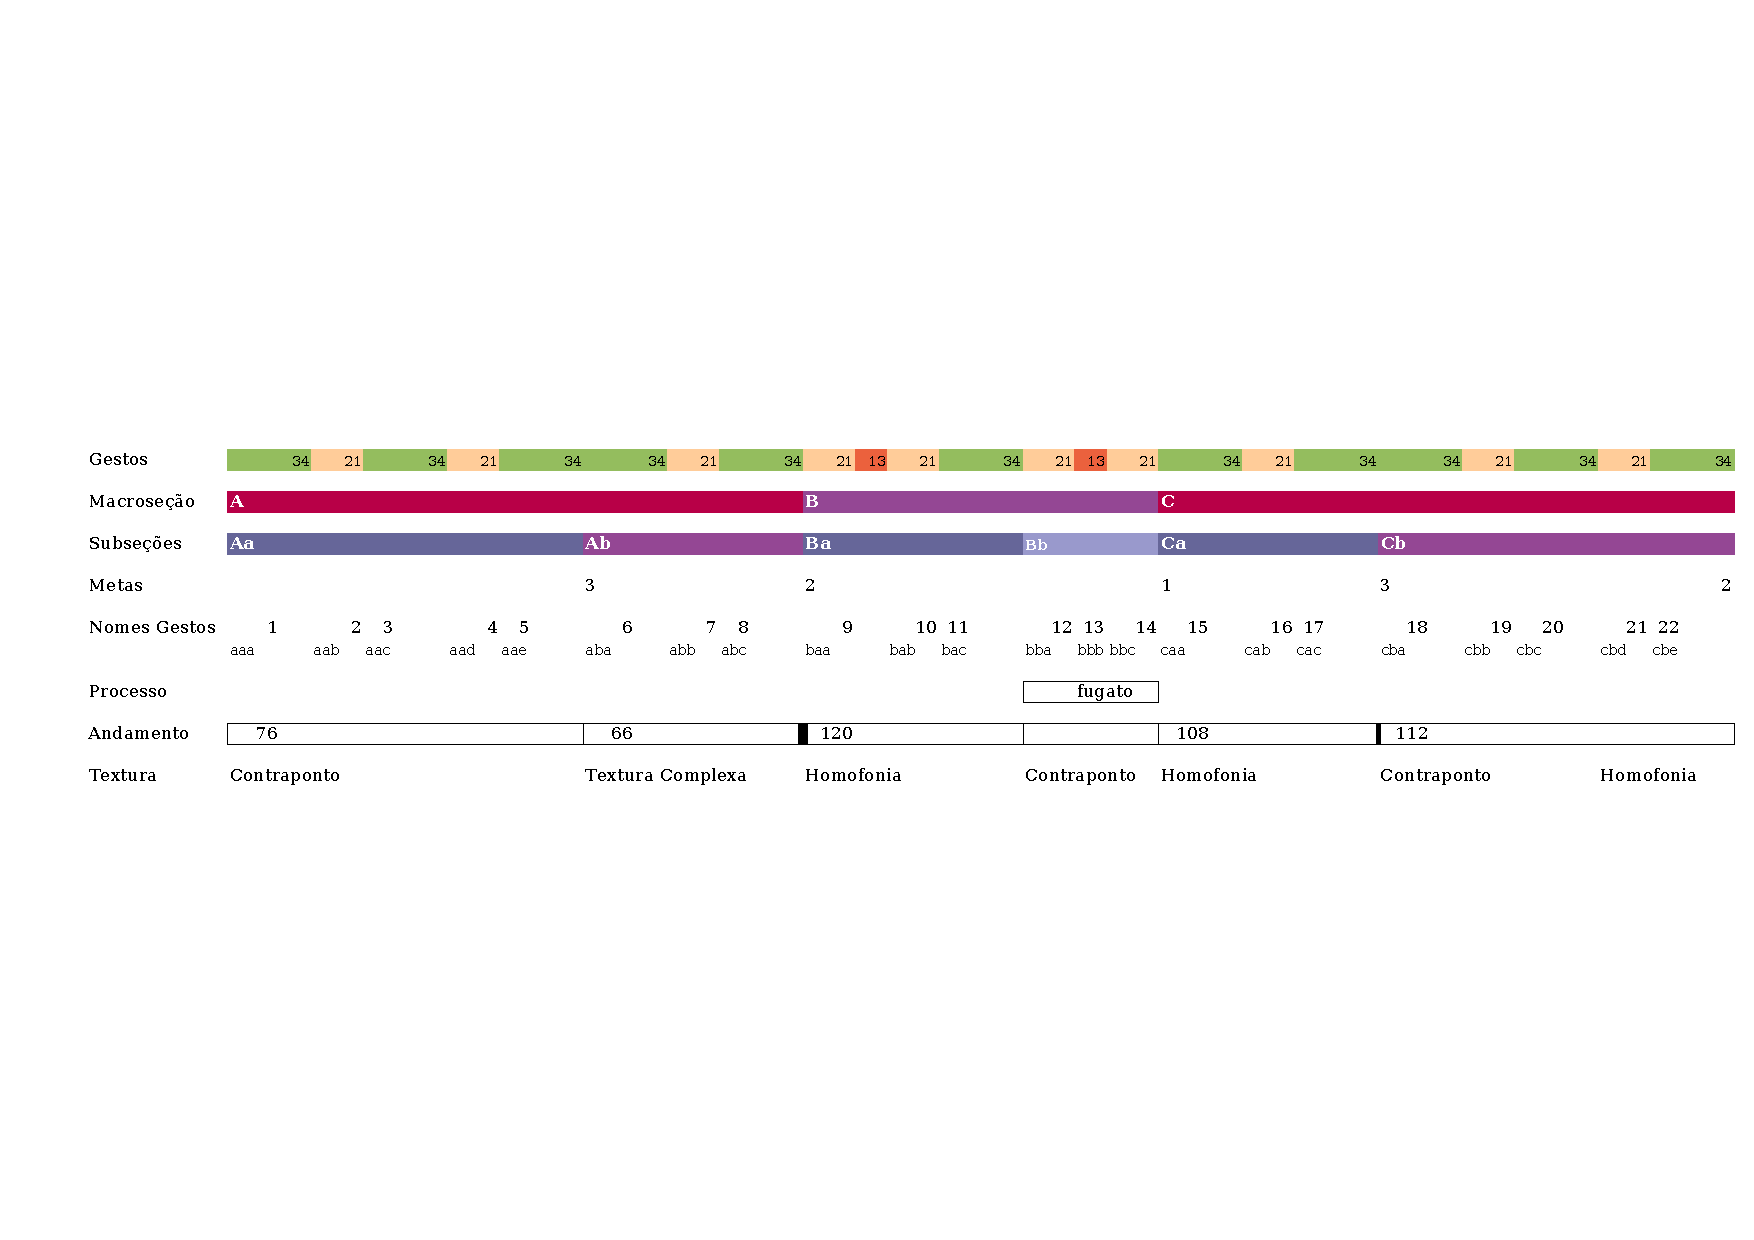
\includegraphics[scale=.81]{planejamento-inicial}
  \caption{Planejamento inicial da peça}
  \label{tab:planejamento-inicial}
\end{table}

No planejamento previmos criar seis seções agrupáveis duas a duas (Aa,
Ab, Ba, Bb, Ca, Cb). Durante a composição dividimos a seção Cb em dois
pedaços, criando então uma nova seção.

As seções menores estão desmembradas em microseções (Aaa, Aab, Aac e
assim por diante). Estas divisões mínimas foram planejadas para conter
microgestos, mas ao longo do processo preferimos trabalhar com gestos
maiores e usá-las para marcar mudanças de instrumental, de timbre, ou
outras intervenções musicais. Além disso os nomes e as numerações dos
gestos ajudaram na organização dos arquivos do Lilypond durante a
composição.

O uso destas microseções para mudança de instrumental pode ser visto
na seção inicial da peça (vide tabela
\ref{tab:microsecoes-primeira-secao}). A microseção Aaa (compassos
1--8) compreende o solo do fagote e tem 29 segundos. a microseção Aab
(compassos 9--14) compreende o trio entre fagote, clarinete e oboé e
tem 22 segundos. A microseção Aac (compassos 15--22), de 29 segundos
compreende o duo entre a melodia inicial no clarinete e o contraponto
da flauta. A microseção Aad (compassos 23--28), de 22 segundos
compreende o quinteto completo. Por último, a microseção Aae
(compassos 29--36), de 29 segundos, compreende o quarteto
fl./ob./cl./fg. e o aumento da densidade.

\begin{table}
  \centering
  \begin{tabular}{r|rrrrr}
    & Aaa & Aab & Aac & Aad & Aae \\
    \hline
    Flauta & & & \cinzaa & \cinzaa & \cinzaa \\
    Oboé & & \cinzab & & \cinzab & \cinzab \\
    Clarinete & & \cinzaa & \cinzaa & \cinzaa & \cinzaa \\
    Trompa & & & & \cinzaa & \cinzaa \\
    Fagote & \cinzab & \cinzab & & \cinzab &
  \end{tabular}
  \caption{Instrumentos utilizados na primeira seção}
  \label{tab:microsecoes-primeira-secao}
\end{table}

Os números 1, 2 e 3 associados às metas representam seu grau de
importância na peça.
%% verificar: gradação ou graduação
Tal graduação porém não foi implementada. Os andamentos foram
levemente modificados para adequação ao material de cada seção. Na
tabela \ref{tab:planejamento-inicial} as barras mais grossas nos
campos dos andamentos representam silêncio entre as seções e não foram
implementadas na versão final. As texturas planejadas foram mantidas
exceto pela seção planejada C (seções 5--7). Neste ponto não há de
fato textura homofônica.

\subsection{Descrição das seções}
\label{sec:descricao-das-secoes}

A seção inicial da obra contém em toda sua extensão a repetição de uma
mesma melodia (vide figura \ref{fig:melodia-inicial}). Esta repetição
é alternada entre os instrumentos. Ainda nesta seção, a partir do
compasso 9, o motivo $\alpha$ (figura \ref{fig:motivo-alfa}) aparece
simultaneamente em duas vozes formando uma textura contrapontística
(vide figura \ref{fig:contraponto-alfa}). O progressivo aumento da
densidade e do nível de dinâmica colaboram com o desenho gestual da
seção, que culmina no acorde do compasso 36.

\begin{figure}
  \centering
  \includegraphics{melodia-inicial}
  \caption{Melodia inicial}
  \label{fig:melodia-inicial}
\end{figure}

\begin{figure}
  \centering
  \includegraphics{contraponto-alfa}
  \caption{Contraponto com motivo $\alpha$}
  \label{fig:contraponto-alfa}
\end{figure}

A segunda seção da obra contém uma textura de entradas defasadas de
notas longas. Estas notas---Si$\flat$2, Mi3, Si$\flat$3 Dó$\sharp$5, e
Sol5---estão em diferentes registros e estão presentes nas linhas de
diferentes instrumentos (vide figura
\ref{fig:contorno-notas-longas}). As maiores características são a
estaticidade das linhas dos instrumentos e o colorido timbrístico. O
seu gestual forma um arco em que a densidade aumenta até um pico, no
compasso 47, e gradativamente descresce (vide figura
\ref{fig:pico-densidade-secao-2}). Esta densidade está relacionada ao
estreitamento e posteriormente ao alargamento das entradas
instrumentais.

\begin{figure}
  \centering
  \includegraphics{contorno-notas-longas}
  \caption{Contorno em textura de notas longas}
  \label{fig:contorno-notas-longas}
\end{figure}

\begin{figure}
  \centering
  %% inserir figura de 3 a 4 compassos seção 2, pico de densidade
  \caption{Pico de densidade na segunda seção}
  \label{fig:pico-densidade-secao-2}
\end{figure}

O início da quarta seção ocorre antes do final da terceira, que tem um
desfecho gradativo, formando uma espécie de dégradé entre estas seções
(vide figura \ref{fig:transicao-3-4}). A quarta seção é um fugato com
sujeito e contra-sujeito derivados do contorno principal e de
combinações de operações\footnote{Para maiores detalhes sobre este
  fugato e combinações de operações vide seção
  \ref{sec:comb-de-oper}.}. Do ponto de vista gestual, há uma passagem
de uma menor densidade no início da quarta seção, com as entradas
instrumentais sucessivas, para uma maior densidade no final da mesma
seção. Isto ocorre por três razões: (1) a entrada da trompa em ritmo
largo (comp. 123), (2) o estreitamento entre as entradas das madeiras,
e (3) a partir do compasso 128, o jogo de perguntas e respostas com o
primeiro segmento do sujeito, que ocorre entre as duplas flauta/fagote
e oboé/clarinete.

\begin{figure}
  \centering
  %% inserir figura de 4 a 5 compassos seção transição seções 3 e 4
  \caption{Transição entre terceira e quarta seções}
  \label{fig:transicao-3-4}
\end{figure}

A quinta seção tem como elemento fundamental um ostinato na linha do
fagote (vide figura \ref{fig:ostinato-fagote}). Este ostinato é
inspirado em um dos toques da capoeira\footnote{A utilização deste
  elemento foi apenas pontual. Por este motivo não aprofundaremos em
  maiores explicações sobre a capoeira e seus toques.}. O ritmo do
ostinato é aproveitado para a construção da bifonia (vide seção
\ref{sec:aspectos-verticais}). O desenho gestual desta seção é
bastante parecido ao da seção inicial, com aumento progressivo da
densidade culminando no acorde do compasso 172.

\begin{figure}
  \centering
  \includegraphics{ostinato-fagote}
  \caption{Ostinato da linha do fagote}
  \label{fig:ostinato-fagote}
\end{figure}

A sexta seção da obra, em contraste às anteriores, é caracterizada por
grupos de notas curtas, rápidas e desligadas. Estes grupos são
separados entre si por silêncios (vide figura
\ref{fig:sexta-secao-184-187}). As linhas dos instrumentos contêm cada
uma o motivo $\alpha$ modificado por operações de
rotação\footnote{Estas operações estão descritas na seção
  \ref{sec:comb-de-oper}.}. Os grupos de notas curtas não englobam
necessariamente todas as notas do motivo $\alpha$. Por vezes o
silêncio interrompe o motivo, como por exemplo na linha da flauta, nos
compassos 177--178 (vide figura
\ref{fig:grupos-separados-silencio}). O motivo é concluído logo após o
silêncio.

\begin{figure}
  \centering
  \subfloat[Textura de notas curtas e silêncios (em dó)]{
    \includegraphics{sexta-secao-184-187}
    \label{fig:sexta-secao-184-187}
  }

  \subfloat[Motivo interrompido por silêncio]{
    \includegraphics{flauta-grupos-silencio}
    \label{fig:grupos-separados-silencio}
  }

  \subfloat[Transição entre os dois gestos da sexta seção]{
    \includegraphics{transicao-sexta-dois-gestos}
    \label{fig:transicao-sexta-dois-gestos}
  }
  \caption{Notas curtas separadas por silêncios (sexta seção)}
  \label{fig:sexta-secao-notas-curtas}
\end{figure}

A sexta seção contém dois gestos interligados. O primeiro gesto
(comp. 173--198) é marcado pelo aumento da densidade, obtido pela
diminuição dos silêncios. O colorido melódico tem destaque no final
deste gesto (comp. 194--198). O segundo gesto (comp. 199--214) é
caracterizado por graduais movimentos ascendentes e movimentação do
âmbito do grave para o agudo. A linha da trompa (comp. 206--215),
derivada da linha do oboé (comp. 149--157) interliga esta seção com a
seguinte. Na figura \ref{fig:transicao-sexta-dois-gestos} percebemos o
início do segundo gesto com elementos do gesto anterior.

A sétima e última seção engloba elementos importantes das seções
anteriores (vide figura \ref{fig:setima-secao-resumo}). A linha do
fagote é uma repetição do que ocorre na quarta seção. A linha do
clarinete representa o ritmo e acentuação da terceira seção. A linha
da trompa corresponde ao solo do fagote do início da peça. As linhas
do oboé e flauta representam a bifonia apresentada na quinta
seção. Finalmente o material apresentado pela flauta e oboé a partir
do compasso 239 representa o sujeito do fugato da quarta seção. As
relações de contornos nesta seção são, portanto, as mesmas que estes
citados elementos mantêm nas seções anteriores.

%% FIXME: refazer figura após terminar composição e inserir colchetes
\begin{figure}
  \centering
  \includegraphics{setima-secao-resumo}
  \caption{Elementos de outras seções na sétima seção}
  \label{fig:setima-secao-resumo}
\end{figure}
\section{Aspectos verticais}
\label{sec:aspectos-verticais}
%% aspectos "harmônicos". melhorar título da seção

A bifonia (figura \ref{fig:bifonia}, p. \pageref{fig:bifonia}) que
origina todo material da peça tem seu conteúdo harmônico derivado da
escala octatônica\footnote{A escala octatônica é obtida a partir da
  superposição de duas das três tétrades diminutas contidas em uma
  escala dodecafônica \cite[p. 76]{antokoletz90:music}.} (figura
\ref{fig:escala-octatonica}).

\begin{figure}
  \centering
  \includegraphics{escala-octatonica}
  \caption{Escala octatônica}
  \label{fig:escala-octatonica}
\end{figure}

Ao longo da obra um acorde é apresentado de forma recorrente (vide
figura \ref{fig:acorde-motivo}). Este acorde é derivado da bifonia e
tem sonoridade octatônica. A terceira seção da peça é inteiramente
construída com este acorde, que tem sua orquestração modificada no
decorrer do gesto.

\begin{figure}
  \centering
  \includegraphics{acorde-motivo}
  \caption{Acorde-motivo}
  \label{fig:acorde-motivo}
\end{figure}

A bifonia é apresentada em sua forma mais explícita na quinta seção
(vide figura \ref{fig:bifonia-grave}). Aparece inicialmente na região
grave, nas linhas do clarinete e da trompa (comp. 137--144), depois
brevemente no oboé e na trompa (comp. 146--149), e mais adiante na
flauta e no clarinete (comp. 157--172).

\begin{figure}
  \centering
  \includegraphics{bifonia-grave}
  \caption{Apresentação da bifonia no clarinete e trompa (ambos em
    dó) c. 137--141}
  \label{fig:bifonia-grave}
\end{figure}
\section{Uso de motivos}
\label{sec:uso-de-motivos}

A obra contém três motivos derivados da bifonia (vide figura
\ref{fig:bifonia}, p. \pageref{fig:bifonia}). O motivo $\alpha$ (vide
figura \ref{fig:motivo-alfa-analisado}) dá origem aos motivos de três
notas $\beta$ (vide figura \ref{fig:motivo-beta}) e de semicolcheias
$\gamma$ (vide figura \ref{fig:motivo-gama}). Além destes há a
presença de um motivo unicamente rítmico $\delta$ (vide figura
\ref{fig:motivo-delta}).

\begin{figure}
  \centering
  \subfloat[Motivo $\beta$]{
    \includegraphics{motivo-beta}
    \label{fig:motivo-beta}
  }
  \subfloat[Motivo $\gamma$]{
    \includegraphics{motivo-gama}
    \label{fig:motivo-gama}
  }

  \subfloat[Motivo $\delta$]{
    \includegraphics{motivo-delta}
    \label{fig:motivo-delta}
  }

  \subfloat[Estrutura do motivo $\alpha$]{
    \includegraphics{motivo-alfa-analisado}
    \label{fig:motivo-alfa-analisado}
  }
  \caption{Motivos utilizados na obra}
  \label{fig:motivos-utilizados}
\end{figure}

O motivo $\alpha$ contém dois motivos $\beta$, um em sua forma
original e outro invertido. Além disso o motivo $\alpha$ também está
presente de forma invertida no motivo $\gamma$, com as notas
Dó-Mi$\flat$-Ré$\flat$. Este motivo $\alpha$ é utilizado na linha do
fagote do início da peça, no sujeito do fugato da quarta seção (letra
L), na linha do clarinete nos compassos 137--144, na linha da flauta
nos compassos 158--171, no material da flauta e oboé na sexta seção
(letra R) e na seção final.
%% inserir figura com linha inicial do fagote
%% inserir seção em que falo que a última seção é resumo das outras

O motivo $\gamma$ é exatamente um retrógrado do motivo $\alpha$ com a
adição do parâmetro duração e da característica anacrúzica. O motivo
está presente na linha do oboé, compasso 149, nas linhas da flauta e
clarinete nos compassos 157--172, na contrução do material ascendente
dos compassos 200--215 e na seção final.

O motivo $\delta$ não tem relação com altura ou contorno. É apenas um
padrão de acentuação que é repetido na terceira e última seções. Na
primeira aparição há notas \eng{stacatto} entre os acentos. Na segunda
aparição há apenas os acentos.

\section{Uso de contornos}
\label{sec:uso-de-contornos}

O objetivo principal da composição da obra \obra{} foi o uso
sistemático de combinações de operações de contorno para a criação
musical. Por isso decidimos escolher um único contorno---de modo a
colaborar com a unidade da peça---e manipulá-lo para gerar a maioria
do material composicional da obra. Escolhemos o contorno de seis
elementos \contpr{}, relacionado com a bifonia e o motivo $\alpha$.

O contorno principal \contpr{} tem forma prima c6-26 (0 2 1 4 3
5)\footnote{A numeração dos contornos (ou segmentos de contornos) pode
  ser vista na tabela de classes de segmentos de contornos
  \cite{marvin.ea87:relating}.}. Este é um contorno simétrico, por
isso retrógrado e inversão são iguais. Este contorno contém
subconjuntos de 5, 4, 3 e 2 elementos.

\subsection{Combinações de operações de contorno utilizadas}
\label{sec:comb-de-oper}

Utilizamos um grupo de operações de contorno e as combinamos para
criar o material musical da obra. Trabalhamos com dois subconjuntos de
contornos, operações de INT$_1$, inversão, rotações e de preenchimento
de contornos. Combinamos estas operações desta forma:

\begin{itemize}
\item Subconjunto com expansão e transposição
\item Interpolação com expansão
\item Rotação com expansão
\item Concatenação de contornos resultando em novo material
\item Rotação com retrogradação
\end{itemize}

%% que termo que usar? melodia? fragmento melódico? motivo?
A combinação das operações de subconjunto, expansão e transposição foi
utilizada na linha do fagote no início da peça. Neste ponto há uma
melodia (vide figura \ref{fig:melodia-inicial},
p. \pageref{fig:melodia-inicial}) construída com o subconjunto do
contorno principal (2 0 1). A melodia tem dois segmentos, sendo o
primeiro derivado das três notas iniciais do motivo $\alpha$, e o
segundo como transposição do segmento anterior com operações de
expansão e transposição. Em ambos os segmentos há preservação do
contorno (2 0 1). Esta melodia está presente em toda a primeira seção
da obra, nos compassos 9--14 no fagote e oboé, nos compassos 15--22 no
clarinete, e nos compassos 23--36 na flauta e trompa.

A combinação de rotação e expansão de contornos ocorre no sujeito e
contra-sujeito do fugato da quarta seção e no material de notas curtas
da sexta seção. O sujeito do fugato (vide figura
\ref{fig:sujeito-fugato}) é constituído por dois segmentos elididos. O
primeiro segmento é o próprio motivo $\alpha$, por consequüencia, é
também o contorno principal (5 3 4 1 2 0). O segundo segmento é o
contorno resultante da combinação da operação de rotação de fator 3,
(1 2 0 5 3 4), e da operação de expansão. O segundo segmento é
iniciado na nota Sol, última nota do segmento anterior.

O contra-sujeito é composto de três segmentos que contêm combinações
de operações de retrogradação e rotação de contornos (vide figura
\ref{fig:contra-sujeito-fugato}). O primeiro segmento contém uma
rotação de fator 5 do retrógrado do contorno principal (5 0 2 1 4
3). A primeira nota está elidida com a última nota do sujeito. O
segundo segmento contém uma rotação de fator 4 do retrógrado do
contorno principal (3 5 0 2 1 4), e também está elidida ao segmento
anterior. Finalmente o terceiro segmento contém uma rotação de fator 3
do retrógrado do contorno principal (4 3 5 0 2 1). Ao contrário dos
outros segmentos, ele não está elidido ao segmento anterior. Pode-se
observar que o contra-sujeito incorpora ainda uma sistemática nas suas
operações de contorno. A cada segmento o fator de rotação diminui em
um ponto.

\begin{figure}
  \centering
  \subfloat[Sujeito]{
    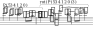
\includegraphics{sujeito-fugato}
    \label{fig:sujeito-fugato}
  }

  \subfloat[Contra-Sujeito]{
    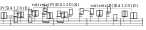
\includegraphics{contra-sujeito-fugato}
    \label{fig:contra-sujeito-fugato}
  }
  \caption{Elementos estruturais do fugato}
  \label{fig:elementos-fugato}
\end{figure}

A combinação de rotação e expansão de contornos também está presente
na sexta seção, nas linhas das quatro madeiras. A linha da flauta
contém o motivo $\alpha$ em sua forma original. A linha do clarinete
contém uma rotação de fator 2 e uma expansão de intervalos de segunda
para intervalos de terça. A linha do oboé contém um desvio da
estrutura do contorno. Trata-se de uma rotação de fator 3 do motivo
$\alpha$, porém com transposição da segunda metade do motivo para uma
oitava abaixo. Neste ponto a estrutura do contorno foi sacrificada em
prol do desenho gestual da seção, que não supera o Ré$\sharp$4 neste
trecho. Finalmente a linha do fagote contém uma rotação de fator 4 do
motivo $\alpha$ e expansão semelhante ao do clarinete. Na figura
\ref{fig:notas-curtas-madeiras} estão exibidas estas variações do
motivo $\alpha$ em cada elemento, na tabela
\ref{tab:operacoes-secao-6} há um esquema com as operações utilizadas
nestas variações, e na figura \ref{fig:rotacoes-534120} estão
representações gráficas das rotações utilizadas.

\begin{figure}
  \centering
    \includegraphics{notas-curtas-madeiras}
    \caption{Operações de rotação e expansão do motivo $\alpha$ na 6ª
    seção}
  \label{fig:notas-curtas-madeiras}
\end{figure}

\begin{figure}
  \centering
  \subfloat[Rotação 2: (4 1 2 0 5 3)]{
    \includegraphics{c-412053}
    \label{fig:412053}  
  }
  \subfloat[Rotação 3: (1 2 0 5 3 4)]{
    \includegraphics{c-120534}
    \label{fig:120534}  
  }
  \subfloat[Rotação 4: (2 0 5 3 4 1)]{
    \includegraphics{c-205341}
    \label{fig:205341}  
  }
  \caption{Rotações no contorno (5 3 4 1 2 0)}
  \label{fig:rotacoes-534120}
\end{figure}

\begin{table}
  \centering
  \begin{tabular}{r|cc}
    Instrumento & Fator de rotação & Expansão \\
    \hline
    Flauta & 0 & Não \\
    Oboé & 3 & Não \\
    Clarinete & 2 & Sim \\
    Fagote & 4 & Sim \\
  \end{tabular}
  \caption{Operações na sexta seção}
  \label{tab:operacoes-secao-6}
\end{table}

A combinação entre expansão e retrogradação ocorre na linha do oboé
nos compassos 149--157 (vide figura \ref{fig:oboe-solo-secao-5}). O
motivo $\gamma$ (vide seção \ref{sec:uso-de-motivos} e figura
\ref{fig:motivo-gama}) é uma retrogradação do motivo $\alpha$ da
peça. Neste trecho este motivo aparece três vezes: na primeira vez em
sua forma original, na segunda vez com uma expansão e intervalo de
segunda para intervalo de terça, e na terça com uma expansão de
intervalo de segunda para intervalo de quarta.

%% inserir análise no inkscape
\begin{figure}
  \centering
  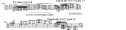
\includegraphics{oboe-solo-secao-5}
  \caption{Solo do oboé na quinta seção}
  \label{fig:oboe-solo-secao-5}
\end{figure}

A combinação entre expansão, rotação, retrógrado e interpolação de
contornos ocorre na linha do oboé nos compassos 149--153. O motivo
$\alpha$ tem uma rotação de fator 3 gerando as notas adjacentes
Sol-Si$\flat$-Lá, e logo após, no compasso 152,
Dó$\sharp$-Si$\sharp$-Ré$\sharp$. Entre estes dois grupos de notas há
uma expansão de intervalos do motivo $\gamma$, iniciado em Dó$\sharp$3
e concluído em Dó$\sharp$4. Como já foi dito, este motivo é uma
retrogradação do motivo $\alpha$. Entendemos que este motivo está
interpolado com o contorno iniciado em Sol.

\subsection{Operações de contornos não combinadas}
\label{sec:cont-nao-comb}

O contorno principal \contpr{} está associado também ao colorido
instrumental. Isto ocorre na segunda seção da peça, em que as
notas---Si$\flat$2, Mi3, Si$\flat$3 Dó$\sharp$5, e Sol5---ocorrem nas
linhas dos instrumentos (vide figura \ref{fig:contorno-notas-longas},
p. \pageref{fig:contorno-notas-longas}).

A operação de INT$_1$ do contorno principal (- + - + -) ocorre de
maneira não ortodoxa no ostinato da linha do fagote, ao longo de toda
a quinta seção (vide figura \ref{fig:ostinato-fagote},
p. \pageref{fig:ostinato-fagote}). O padrão com as notas Sol e Lá
sugere o movimento (- +) presente no contorno principal.

%% falar sobre o gestual da quinta seção e uso da anacruze e da
%% semelhança com o contraponto da primeira seção

\subsection{Contornos associados a outros parâmetros musicais}
\label{sec:cont-assoc-outr}

Contornos estão associados a outros parâmetros musicais como
andamento, densidade e textura.

Os andamentos utilizados na peça---82, 66, 120, 108 e 112 (vide tabela
\ref{tab:secoes-obra}, p. \pageref{tab:secoes-obra})---representam o
contorno A(1 0 4 2 3). Este contorno é um subconjunto de 5 elementos
do contorno principal utilizado, \contpr{}.

Na seção inicial da obra relações de contornos estão associados a
densidade. A densidade neste trecho tem contorno D(1 3 2 5 4), isto é
começa com um instrumento, depois um trio, um duo, o quinteto completo
e um quarteto. Esta seção é iniciada com um solo de fagote (1) seguido
de um trio com fagote, clarinete e oboé (3). Ocorre então um duo entre
clarinete e flauta (2), um \eng{tutti} (5) e finalmente um quarteto
sem o fagote (4). Este contorno D é o retrógrado de um subconjunto de
5 elementos do contorno principal P.

As texturas presentes na peça podem ser divididas em dois grandes
grupos: de texturas homofônicas, que engloba texturas corais e de
melodia acompanhada; e de texturas polifônicas, que engloba textura
contrapontística e textura complexa. Estes grupos são apresentados
nesta ordem:
polifonia-homofonia-polifonia-homofonia-polifonia-homofonia. Considerando
que uma textura polifônica é mais complexa que uma textura homofônica,
a alternância entre estas texturas delineia um contorno de INT$_1$ (-
+ - + -), derivado do contorno principal \contpr{}.

\subsection{Operações de contorno não utilizadas}
\label{sec:oper-de-cont}

Nem todas as operações das teorias de contornos foram utilizadas na
composição. A \tr{COM-matrix}, por exemplo, é bastante utilizada para
análise, mas não encontramos uma forma interessante de usá-la na
composição.

\begin{figure}
  \centering
  \begin{tabular}{r|cccccc}
      & 5 & 3 & 4 & 1 & 2 & 0 \\
      \hline
    5 & 0 & - & - & - & - & - \\
    3 & + & 0 & + & - & - & - \\
    4 & + & - & 0 & - & - & - \\
    1 & + & + & + & 0 & + & - \\
    2 & + & + & + & - & 0 & - \\
    0 & + & + & + & + & + & 0
  \end{tabular}
  \caption{Matriz de comparação do contorno (5 3 4 1 2 0)}
  \label{fig:matriz-534120}
\end{figure}


\chapter{Conclusão}
\label{cha:conclusao}
